\documentclass[12pt]{article}

% Math and symbol packages
\usepackage{amsmath}
\usepackage{amssymb}
\usepackage{derivative}

% Figure Packages
\usepackage{graphicx}
\usepackage{wrapfig}
\usepackage{epstopdf}
\usepackage{float}
\usepackage{subfigure}

% Formatting and Random Text Generation
\usepackage{inputenc}
\usepackage[left=2.54cm,right=2.54cm,top=2.54cm,bottom=2.54cm]{geometry}
\usepackage{lipsum}

% Header and indent packages
\usepackage{fancyhdr}
\usepackage{indentfirst}

% Create Title Section
\title{Rotational Kinetic Energy}
\author{Trevor Swan \\
Department of Physics, Case Western Reserve University \\
Cleveland, OH 44016-7079}
\date{}

% Create paragraph formatting
%\setlength{\parindent}{3em}

% Actual Lab content
\begin{document}
\pagestyle{fancy}
\fancyhf{}

% Load the title
\maketitle
\thispagestyle{fancy}
\renewcommand{\headrulewidth}{0pt}

% Set up Footers
\fancyfoot[L]{Trevor Swan}
\fancyfoot[C]{\thepage}
\fancyfoot[R]{Rotational Kinetic Energy}

% Abstract section of Report
\section{Abstract}
By using a \textit{Roto-Dyne} wheel and the Conservation of Energy, I have derived  the moment of inertia for a rotating object with 4 fixed point masses a constant distance from the pivot point. I created a Monte Carlo simulation in \textit{Origin} to develop a working model to analyze data generated from a hanging mass falling from a string attached to an apparatus. My preliminary calculations generated a theoretical moment of inertia of $J=0.045\ kg\cdot m^2$, which supported the result of the actual simulation of $I=0.0450\ kg\cdot m^2$. I then used the simulation to analyze data generated from dropping a hanging mass off of a wheel with and without the point masses attached. These data were collected using the \textit{Logger Pro} software. I calculated the moment of inertia with the point masses to be $I_1=0.0724\ kg\cdot m^2$ and $I_2=0.0338\ kg\cdot m^2$ for the wheel without the point masses. The difference of these values represents the experimental value of the moment of inertia for the mass loads, which I calculated to be $I_E=0.0386\pm0.0005\ kg\cdot m^2$. I then predicted value for the moment of inertia for the 4 masses as $I_P=0.0271\pm0.0003\ kg\cdot m^2$. These values do not agree as a result of large amounts of systematic error in my experiment.

% Introduction and Thoery

\section{Introduction and Theory}
The Conservation of Energy can be used to derive the moment of inertia of a given object by utilizing rotational and transnational kinetic energy. The moment of inertia of a point object rotating in a circle can be calculated given a mass $M$ and a radius $R$ with the equation: \par

% Basic inertia equation
\begin{equation}
    I=MR^2 \label{Inertia}
\end{equation}

\indent For non-point object's, the moment of inertia is dependent on the object's actual shape. In the case of a disk, this expression is:

% Inertia equation for a disk
\begin{equation}
    I_{\text{disk}}=\frac{1}{2}M_{\text{disk}}R^2 \label{disk}
\end{equation}

\indent We are also interested in the moment of inertia for rings, which is:

% Inertia equation for a ring
\begin{equation}
    I_{\text{ring}}=M_{\text{ring}}R^2 \label{ring}
\end{equation}

\indent The \textit{Roto-Dyne} wheel used in this experiment is neither a disk or a ring, as it is not either hollow or completely filled in. The wheel shares characteristics of both objects, as seen in Figure \ref{apparatus}. Despite this observation, we can safely assume that the moment of inertia lies between the expressions listed in Equations \ref{disk} and \ref{ring}. \par 

Our experiment contends with both transnational and rotational kinetic energy. The kinetic energy of an object with mass $M$ and transnational speed $v$ is:

% Trans Kinetic Energy Equation
\begin{equation}
    K_T=\frac{1}{2}Mv^2 \label{trans}
\end{equation}

\indent For a rotating object with a given moment of inertia $I$ and angular speed $\omega$ is a similar expression given by:

% Rotational Kinetic Energy Equation
\begin{equation}
    K_R=\frac{1}{2}I\omega^2 \label{rot}
\end{equation}


\indent We can define the $y=0$ point as the plane level with the wheel seen in Figure \ref{apparatus}. Assuming the hanging mass drops a distance $y$ from this initial point, its potential energy, $\Delta U_W$,is decreased as its kinetic energy, as seen in Equations \ref{trans} and \ref{rot}, increases. The total sum of the energy can be compared to the total work done by friction in the following equation:

% Conservation of energy
\begin{equation}
    \Delta U_W+K_T+K_R=W_f \label{CofME}
\end{equation}

\indent As explained in the experimental procedure, we added a small mass $m$ to the string of the apparatus to overcome the $W_f$ term. This mass, however, is negligible when compared to the hanging mass. Substituting Equations \ref{trans} and \ref{rot} into Equation \ref{CofME} along with 0 work done by friction yields:

% CofME substituted
\begin{equation}
    \Delta U_W+\frac{1}{2}Mv^2+\frac{1}{2}I\omega^2=0
\end{equation}

\indent We can let the positive y direction be defined as everything below the wheel. This allows us to substitute $-Mgy$ in for $\Delta U_W$ and $\omega = \frac{v}{r}$ via the rolling constraint. We can then derive a set of functionally equivalent equations:

% Define and align important equations
\begin{align}
    0=&-Mgy+\frac{1}{2}Mv^2+\frac{1}{2}I(\frac{v}{r})^2 && \text{Substitute Givens} \label{substitute} \\
    Mgy=&\frac{1}{2}[M+\frac{I}{r^2}]v^2 && \text{Rearrange} \label{rearrange} \\
    gy=&\frac{1}{2}[1+\frac{I}{Mr^2}]v^2 \label{gy} && \text{Solve for }gy
\end{align}

\indent Analyzing our data involves comparing $v^2$ against $y$ in a plot. We can say y is the independent variable, so we must express Equation \ref{gy} as $v^2$ in terms of $y$:

% Express v^2 in terms of y
\begin{equation}
    v^2 = \frac{2gyMr^2}{Mr^2+I} \label{slope}
\end{equation}

\noindent It should be noted that we expect the line generated by a plot of $v^2$ vs. $y$ to be roughly linear.

\indent More functionally, we can solve Equation \ref{gy} for $I$, which can be used for further analysis in our experimental procedure. The algebra that leads up to this equation is unnecessary to present here, but it simplifies to the following:

% Inertia Equation based on CofME
\begin{equation}
    I=Mr^2(\frac{2gy}{v^2}-1) \label{I of CofME}
\end{equation}

\indent For the Monte Carlo part of our experiment, we had to determine a value for $\Delta t$. To do this we need to emphasize the following relationship:

% Velocity Approx
\begin{equation}
    v=\frac{\Delta s}{\Delta t} \label{v approx}
\end{equation}

\noindent Where $s$ is the value reported by \textit{Logger Pro} based on when the gate is on and off. \par
\indent We can then use Equation \ref{v approx} in conjunction with Equation \ref{gy} to solve for $\Delta t$, yielding the following useful relationship:

% dt0 expression
\begin{equation}
    \Delta t = \Delta s*\sqrt{\frac{1+I}{2gyMr^2}} \label{dtr}
\end{equation}

\indent For the actual experiment, we had to contend with actual uncertainties in $v^2$, or $\delta_{v^2_t}$. We can use the following equation to calculate the uncertainty in velocity due to time in \textit{Origin}. While this is related to any real error analysis, it is useful in determining the error bars for Figures \ref{Massed Plot} and \ref{Massless Plot}. The equation is derived from squaring Equation \ref{v approx} as follows:

% Show the derivation of v^2_t
\begin{equation}
    \begin{split}
        \delta_{v^2_t}=\frac{\partial}{\partial \Delta t}(\frac{\Delta s^2}{\Delta t^2})*\delta_{\Delta t} = 2\frac{\Delta s^2}{\Delta t^3}\delta_{\Delta t}=2\frac{\Delta s^2}{\Delta t^3}\frac{\Delta s}{\Delta s}*\delta_{\Delta t}=2\frac{v^3}{\Delta s}*\delta_{\Delta t}
    \end{split}
\end{equation}

\noindent This equation will not be used or referenced again in this paper, and serves only to illustrate our method for developing error bars for Figures \ref{Massed Plot} and \ref{Massless Plot}.

% Procedure
\section{Experimental Procedure}
% This paragraph talks about the Monte Carlo Simulation
We started our experiment by creating a Monte Carlo Simulation to generate a model set of data. This first half of the experiment allowed us to create a random set of data for the apparatus shown in Figure \ref{apparatus}. We then seeded random data using the number 0831, and also used the value $\Delta t=0.002$ to run our simulation. To ensure that our data was in fact random as per the Gaussian Distribution, we ran the generator 4 times, yielding 4 different values each time. Knowing that our simulation was successful, we then moved on to the actual part of the experiment. \par

% Insert the Image of the apparatus
\begin{wrapfigure}{R}{0.5\textwidth}
  \begin{center}
    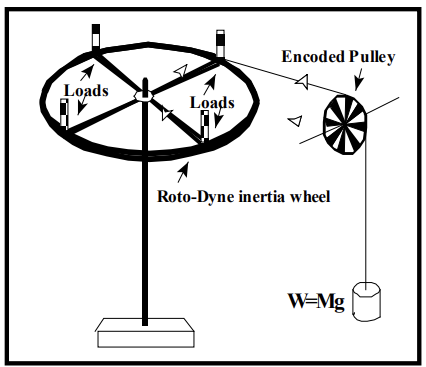
\includegraphics[width=0.48\textwidth]{Experimental Apparatus.png}
  \end{center}
  \caption{Experimental Apparatus}
  \label{apparatus}
\end{wrapfigure}

% This paragraph is about the preliminary measurements of the apparatus
For the latter half of this experiment, we operated the actual apparatus in Figure \ref{apparatus}. It is made up of a \textit{Roto-Dyne} inertia wheel of given mass $M_r=1.5kg$. Although the masses of the detachable weights were given to us, we measured them with the Lab's scale, yielding a combined weight of $0.9254\pm 0.0001kg$. We chose this uncertainty because the scale is only accurate up to the tenths place in grams. This differed from the expected value of $0.225\pm0.002kg$ per weight, so we decided to use our measured value for all following calculations. We then measured the radius of the apparatus' wheel by measuring the diameter and then dividing by 2. This yielded a radius of $r=0.209\pm0.001m$, which differed from the given radius of $r_{\text{given}}=0.200\pm0.002m$. We then approximated the radial distance from the center of the Mass Loads to the center of the wheel as $k=0.171\pm0.001m$ by subtracting 3 Load Radii of $r_{\text{load}}=0.0126m$ from the total wheel radius. Note that we chose the uncertainty in our measurement because our meter stick is only accurate to one decimal place in millimeters. \par

% This paragraph talks about the 'massless' experiment
After recording these measurements, we preceded onto the experiment involving no masses on the wheel itself. Before we recorded any data, we had to contend with the frictional force exerted by the string on the encoded pulley. To neglect the force of friction, we added $0.0009kg$ worth of paper clips to the hanging weight. This mass will \textit{not} be included in any future calculations. We knew this mass was correct as the wheel moved at a constant velocity after a gentle push, as verified by \textit{Logger Pro}. We then added the proper hanging mass of $M=0.060kg$ to the string, and dropped it after winding up the wheel. Using \textit{Logger Pro}, we recorded a good set of data and saved it for further use. \par

% This paragraph talks about the 'massed' experiment
Finally, we repeated the above process, though this time we secured the 4 detachable masses on the wheel. Following the exact same procedure, we found that a paperclip mass of $0.0015kg$ was adequate, though this value will be neglected in further calculations. We then added the hanging mass of $M=0.060kg$ back on the apparatus, and recorded data using \textit{Logger Pro} once again.

% This paragraph briefly discusses uncertainty
We will only consider uncertainties in the radius for the apparatus, as well as the uncertainty in the summed mass of the detachable weights. It is safe to neglect the uncertainties in the other components of this system such as the Hanging Mass, as they make use of finely machined parts.


% Results and Analysis
\section{Results and Analysis}
First we analyzed the Monte Carlo experiment to ensure our experimental design wasn't flawed. We had to first estimate a the moment of inertia for the wheel. As the wheel shares characteristics of both a ring and a disk, we can define a moment of Inertia $J$ as:

% Inertia J
\begin{equation}
    \begin{split}
        J=&\frac{I_{disk}+I_{ring}}{2} \\
        =&\frac{MR^2+\frac{1}{2}MR^2}{2} \\
        =&\frac{3}{4}MR^2 \label{J} \\
    \end{split}
\end{equation}

\noindent Note that $J$ is used above to avoid confusion in the simulation. It is derived by using Equations \ref{disk} and \ref{ring}. \par
We can then solve for $J$ using a given mass $M=1.5kg$ and radius $R=0.2m$. This yields the following:

% Unnumbered, calculation of J only
\begin{equation*}
    J=\frac{3}{4}*(1.5kg)*(0.2m)^2=0.045\ kg\cdot m^2
\end{equation*}

\indent We analyzed our simulation by plotting $v^2$ against $y$. While $y$ was generated using an \textit{Origin} script, we had to calculate $v^2$ using the following:

% State the equation used for v^2
\begin{equation}
    v^2=(\frac{0.015}{\Delta t})^2 \label{MC v}
\end{equation}

\noindent With $\Delta t$ be defined by Equation \ref{dtr}. \par

We needed to conduct analysis on Equation \ref{MC v} which required finding the uncertainty in $v^2$. There is only one variable in this equation, so the uncertainty in $v^2$ can be represented by the following expression:

% Uncertainty for v^2
\begin{equation}
    \delta_{v^2}=\sqrt{\delta_{v^2_{\Delta t}}^2} \label{UNC v MC}
\end{equation}

\noindent Where we have to find the value $\delta_{v^2_{\Delta t}}$. \par

The uncertainty in velocity squared due to $\Delta t$ can be calculated using the derivative method as follows:

% Derivative calculation 
\begin{equation}
    \begin{split}
        \delta_{v^2_{\Delta t}}=\frac{\partial v^2}{\partial \Delta t}*\delta_{\Delta t}
        =&\frac{\partial}{\partial\Delta t}(\frac{0.015}{\Delta t})^2*\delta_{\Delta t} \\
        =&\frac{-2(0.015)^2}{(\Delta t)^3}*\delta_{\Delta t} \label{v derivative MC}
    \end{split}
\end{equation}

\noindent The above equation can be plugged into Equation \ref{UNC v MC}, Effectively taking the absolute value of the expression. $\Delta t$ is evaluated dynamically, as it changes based on the inputted simulation. The given value for $\delta_{\Delta t}$ is $0.0002$ sec, which we will plug into the expression, however:

% Finish the Uncertainty Calculation
\begin{equation}
    \delta_{v^2}= \frac{2(0.015)^2}{(\Delta t)^3}*0.0002 \label{MC UNC}
\end{equation}

\indent We then plotted $v^2$ against $y$ making use of the error bars produced from Equation \ref{MC UNC}. As seen in Figure \ref{MC Plot}, all of our simulated data points' error bars contain the best fit line generated from \textit{Origin}. We expected this result because this data was purely a simulation, and any discrepancies would be a result of poor calculations, not experimental errors. The slope of the generated fit line, as seen in Figure \ref{MC UNC}, is $B=0.993\pm0.002\frac{m}{s^2}$. \par

We can rewrite $B$, the slope of the line, in terms of $y$ and $v^2$ to justify the substitution of $B$ into Equation \ref{I of CofME}. This expression is $B=\frac{y}{v^2}$, whose substitution leads to the following expression:

% Inertia in terms of B
\begin{equation}
    I=Mr^2[\frac{2g}{B}-1] \label{I in B}
\end{equation}

\noindent Plugging $g=9.81\frac{m}{s^2},M=0.060\ kg,r=0.2m, B = 0.993,\text{ and}, \delta_{B}=0.002$ into Equation \ref{I in B} reveals the following value for $I$:

% Final calculation for I
\begin{equation*}
    I=0.06(0.2)^2[\frac{2(9.81)}{0.993}-1]=0.0450
\end{equation*}

\indent To conduct error analysis on $I$, we should contend with uncertainties in both the radius $r$ and in the slope $B$. For the simulation, however, we only need to contend with the uncertainty in $B$ as the uncertainty in $I$ due to $r$ is assumed to be negligible. Therefore, the uncertainty in $I$ can be represented by the following equation:

% Full uncertainty in I
\begin{equation}
    \delta_I=\sqrt{\delta_{I_B}^2} \label{unc in I}
\end{equation}
\indent We only need to contend with the uncertainty in $B$ for the Monte Carlo simulation, the uncertainty in I is represented by effectively taking the absolute value of $\delta_{I_B}$, as seen here:

% Present to component of the uncertainty in I
\begin{equation}
    \begin{split}
        \delta_{I_B}=\frac{\partial I}{\partial B} *\delta_{B}=&\frac{\partial}{\partial B}(Mr^2(\frac{2g}{B}-1))*\delta_{B}  \\
        =&\frac{-2gMr^2}{B^2}*\delta_{B} \label{dIB}
    \end{split}
\end{equation}

\noindent Using this Equation along with Equation \ref{unc in I} and plugging identical values as the preliminary moment of inertia calculation yields the value:\par

% Final caluclation for I_B
\begin{equation*}
    \delta_I =\sqrt{(\frac{-2(9.81)(0.06)(0.2)^2}{0.993^2}*0.002)^2}=0.000112
\end{equation*}

\indent We can then express our value for $I$, rounded correctly with its uncertainty, as $I=0.0450\pm0.0001\ kg\cdot m^2$. This value perfectly aligns with the calculated value derived from Equation \ref{J} of 0.0450$kg\cdot m^2$. We can therefore conclude that our simulation and analysis procedure is correct, so we can now analyze the produced data from the actual trials. \par

Knowing that our method of analysis was correct, we then applied it to the actual data. First, we examined the trial with the 4 masses on the apparatus. As outlined in the procedure, we used a $0.06\ kg$ hanging mass to conduct this test. We plotted the results produced from our software as a plot of $v^2$ against $y$. The outputted slope is $B_1=0.685\pm0.003\ \frac{m}{s^2}$, as verified by Figure \ref{Massed Plot}. \par

We then proceeded to test without the masses on the wheel, while maintaining the same $0.06\ kg$ mass as indicated in the procedure. We made a similar plot as that of the trial with mass, and reported the slope and its uncertainty. For this experiment, we recorded a slope of $B_2 = 1.410\pm0.003\frac{m}{s^2}$, as verified by Figure \ref{Massless Plot}. \par

With two usable slopes, we then plugged them into Equation \ref{I in B} to generate their corresponding values of I, appropriately named $I_1$ for slope $B_1$, and $I_2$ for slope $B_2$. As we operated the actual equipment, we used actual measurements as opposed to the theoretical ones used in the Monte Carlo simulation. This means that we used our measured radius of $r=0.209m$ and hanging mass weight $M=0.06kg$. Plugging the previously stated values of B into their respective equations with respect to both Equation \ref{I in B} and given constants, we yielded the two following values for I:

% Calculations for experimental I values
\begin{align*}
    I_1 =& 0.06(0.209)^2[\frac{2(9.81)}{0.685}-1]=0.0724\ kg\cdot m^2 \\
    I_2 =& 0.06(0.209)^2[\frac{2(9.81)}{1.410}-1]=0.0338\ kg\cdot m^2
\end{align*}

\indent With the two values of $I$ calculated, we then proceeded to calculate the experimental value of the moment inertia for the \textbf{mass loads alone}, as that is what we are ultimately interested in. The relationship is as follows:

% I_E expression
\begin{equation}
    I_E = I_1-I_2 \label{exp I}
\end{equation}

We can substitute the values of $I_1$ and $I_2$ into Equation \ref{exp I}, yielding:

% Calculate the moment of inertia for the mass loads
\begin{equation*}
    I_E=0.724-0.338=0.0386\ kg\cdot m^2
\end{equation*}

\indent We must now contend with the uncertainties in $I$ as a result of $B$ and $r$. Substituting Equation \ref{I in B} into Equation \ref{exp I} with the appropriate values of $B$ allows us to conduct error analysis. This substitution and following simplification is as follows: 

% Substituted I values
\begin{equation}
    \begin{split}
        I_E=&Mr^2[\frac{2g}{B_1}-1] - Mr^2[\frac{2g}{B_2}-1] \\ 
        =& 2gMr^2[\frac{1}{B_1}-\frac{1}{B_2}] \label{IE Simple}
    \end{split}
\end{equation}

\indent We can neglect uncertainties in $M$ and $g$, as these values are either negligible in their own uncertainties or given constants, respectively. This means we can find the uncertainty in $I_E$, or $\delta_{I_E}$, with the following expression:

% Express uncertainty expression for I_E
\begin{equation}
    \delta_{I_E}=\sqrt{\delta^2_{I_{E,B_1}}+\delta^2_{I_{E,B_2}}+\delta^2_{I_{E,r}}} \label{UNC in IE}
\end{equation}

\indent Making use of the derivative method and Equation \ref{IE Simple}, we can derive expressions for $\delta_{I_{E,B_1}}$, $\delta_{I_{E,B_2}}$, and $\delta_{I_{E,r}}$ as follows:

% Express uncertainty in the three quantities that make up IE
\begin{align}
    % due to B_1
    \begin{split}
        \delta_{I_{E,B_1}}= \frac{\partial I_E}{\partial B_1}*\delta_{B_1}=&\frac{\partial}{\partial B_1}(2gMr^2[\frac{1}{B_1}-\frac{1}{B_2}])*\delta_{B_1} \\
        =& \frac{-2gMr^2}{(B_1)^2}*\delta_{B_1} \label{I due B1}
    \end{split} \\ \nonumber \\
    % due to B_2
    \begin{split}
        \delta_{I_{E,B_2}}= \frac{\partial I_E}{\partial B_2}*\delta_{B_2}=&\frac{\partial}{\partial B_2}(2gMr^2[\frac{1}{B_1}-\frac{1}{B_2}])*\delta_{B_2} \\
        =& \frac{2gMr^2}{(B_2)^2}*\delta_{B_2} \label{I due B2}
    \end{split} \\ \nonumber \\
    % due to r
    \begin{split}
        \delta_{I_{E,r}}= \frac{\partial I_E}{\partial r}*\delta_{r}=&\frac{\partial}{\partial r}(2gMr^2[\frac{1}{B_1}-\frac{1}{B_2}])*\delta_{r} \\
        =& 4gMr[\frac{1}{B_1}-\frac{1}{B_2}]*\delta_r \label{I due r}
    \end{split}
\end{align}

\indent We can then compute the values of these individual uncertainties based on given values. For the following calculations, we will use the same values as used in the calculation of the individual Inertia Calculations. In addition, we will use $\delta_{B_1}=0.003$, $\delta_{B_2}=0.003$, and $\delta_r=0.001$ as discussed previously. Substituting appropriate values into Equations \ref{I due B1}, \ref{I due B2}, and \ref{I due r} yields:

% Calculations for uncertianties
\begin{align*}
    % due to B_1
    \begin{split}
        \delta_{I_{E,B_1}}=\frac{-2(9.81)(0.06)(.209)^2}{0.685^2}*.003=-3.29\times10^{-4}
    \end{split} \\ \\
    % due to B_2
    \begin{split}
        \delta_{I_{E,B_2}}=\frac{2(9.81)(0.06)(0.209)^2}{1.410^2}*0.003=7.76\times10^{-5}
    \end{split} \\ \\
    %due to r
    \begin{split}
        \delta_{I_{E,r}}=4(9.81)(0.06)(0.209)[\frac{1}{0.685}-\frac{1}{1.410}]*0.001=3.69\times10^{-4}
    \end{split}
\end{align*}

\indent We can then plug these calculated values into Equation \ref{UNC in IE} to yield the following value of $\delta_{I_E}$:

% Caluclation for true IE unc
\begin{equation*}
    \delta_{I_E}=\sqrt{(-3.29\times10^{-4})^2+(7.76\times10^{-5})^2+(3.69\times10^{-4})^2}=5\times10^{-4}=0.0005\ kg\cdot m^2
\end{equation*}

\indent Using this calculation, we can then express $I_E$ with its uncertainty as $I_E=0.0386\pm0.0005\ kg\cdot m^2$. \par

Now we must contend with the predicted moment of inertia for the \textbf{mass loads alone}. If we treat the Mass Loads as point particles of combined mass $M$ at a distance $k$ from the center of rotation, then we can say that their predicted moment of inertia is as follows:

% Predicted moment of inertia
\begin{equation}
    I_P = Mk^2 \label{predicted moment}
\end{equation}

\noindent Where $M=0.9254kg$ and $k=0.171m$. We can solve this equation with the inputted values stated previously, yielding a predicted moment of inertia for the Load Masses of:

% Calculate I_P
\begin{equation*}
    I_P=0.9254(0.171)^2=0.0271\ kg\cdot m^2
\end{equation*}

We must now perform error analysis on $I_P$, where uncertainty is a result of both $M$ and $k$. The expression for the uncertainty is very similar to the format of Equation \ref{unc in I}, with the individual quantities being added in quadrature. The expression is as follows:

% Uncertainty in I_P
\begin{equation}
    \delta_{I_P}=\sqrt{\delta^2_{I_P,M}+\delta^2_{I_P,k}} \label{UNC in p}
\end{equation}

\indent Once again we will use the derivative method and Equation \ref{predicted moment} to derive the components of this calculation:

% Symbolic Expressions for Uncertainties
\begin{align}
    % IP due to M
    \begin{split}
        \delta_{I_P,M}=\frac{\partial I_P}{\partial M} * \delta_M=&\frac{\partial}{\partial M}(Mk^2)*\delta_M \\
        =&k^2*\delta_M \label{IP due M}
    \end{split} \\ \nonumber \\
    % IP due to k
    \begin{split}
        \delta_{I_P,k}=\frac{\partial I_P}{\partial k}*\delta_k=&\frac{\partial}{\partial k}(Mk^2)*\delta_k \\
        =&2Mk*\delta_k \label{IP due k}
    \end{split}
\end{align}

\indent We can then numerically evaluate these expressions using the same values of $M$ and $k$ used to calculate $I_P$ in Equation \ref{predicted moment}. We will also use $\delta_M=0.0001\ kg$ and $\delta_k=0.001\ m$ as discussed in the Procedure. Plugging these values into Equations \ref{IP due M} and \ref{IP due k} results in the following calculations:

% Actually calculate components of uncertainty
\begin{align*}
    % IP in M
    \begin{split}
        \delta_{I_P,M}=0.171^2*0.0001=2.92\times10^{-6}
    \end{split} \\ \\
    % IP in k
    \begin{split}
        \delta_{I_P,k}=2(0.9254)(0.171)*0.001=3.16\times10^{-4}
    \end{split}
\end{align*}

\indent We can then plug these values into Equation \ref{UNC in p} to yield the following value of $\delta_{I_P}$:

% Calculate I_P true unc
\begin{equation*}
    \delta_{I_P}=\sqrt{(2.92\times10^{-6})^2+(3.16\times10^{-4})^2}=3.16\times10^-4=0.000316\ ks\cdot m^2
\end{equation*}

\indent We can then combine our calculations that made use of Equations \ref{predicted moment} and \ref{UNC in p} to present $I_P$ with its uncertainty as $I_P=0.0271\pm0.0003\ kg\cdot m^2$. \par

Our values of $I_E$ and $I_P$ do not agree within their uncertainties, so we can conclude that a source of systematic error may have been present, or that one or more of our assumptions were incorrect moving through our testing and analysis process.

% Conclusion
\section{Conclusion}
The expected value for the moment of inertia of the 4 Mass Loads was $I_P=0.0271\pm0.0003\ kg\cdot m^2$. The measured value of the moment of inertia was $I_E=0.0386\pm0.0005\ kg\cdot m^2$. These two values do not agree within their uncertainties, with $I_E$ being 23 standard deviations above $I_P$. The reason for this large error is most likely a result of systematic errors in our data collection. This hypothesis is supported by the fit lines in Figures \ref{Massed Plot} and \ref{Massless Plot}. Some of the data points have error bars that do not capture the line of best fit. The data tends to be overestimated by the fit line, suggesting systematic error in our procedure. This could be a result of the \textit{Roto-Dyne} wheel not being perfectly level resulting in artificial acceleration, or from a lack of proper adjustment of friction in our preliminary setup. Also, our estimate of $k$ may have resulted in an incorrect value for $I_P$, though we can confidently say that our estimate was close enough to not alter our prediction too significantly. Finally, we may have treated the release of the hanging mass incorrectly, potentially starting from different points for the trials with and without mass, respectively. All of these factors came together to produce large, systematic error leading to the discrepancies in our results. Ultimately, we cannot develop an accurate representation for the moment of inertia regarding our apparatus, involving a system with 4 evenly spaced point masses.

\subsection{Acknowledgements}
I would like to thank Adi Mallik, CWRU Department of Physics, for his help in obtaining the experimental data, preparing the figures, and checking my calculations.

\subsection{References}
\begin{enumerate}
    \item Driscoll, D., General Physics I: Mechanics Lab Manual, “Rotational Kinetic Energy,” CWRU Bookstore, 2014.
\end{enumerate}

% Appendix to organize plots of data
\clearpage
\section{Appendix}
% Display the MC Plot
\begin{figure}[H]
    \centering
    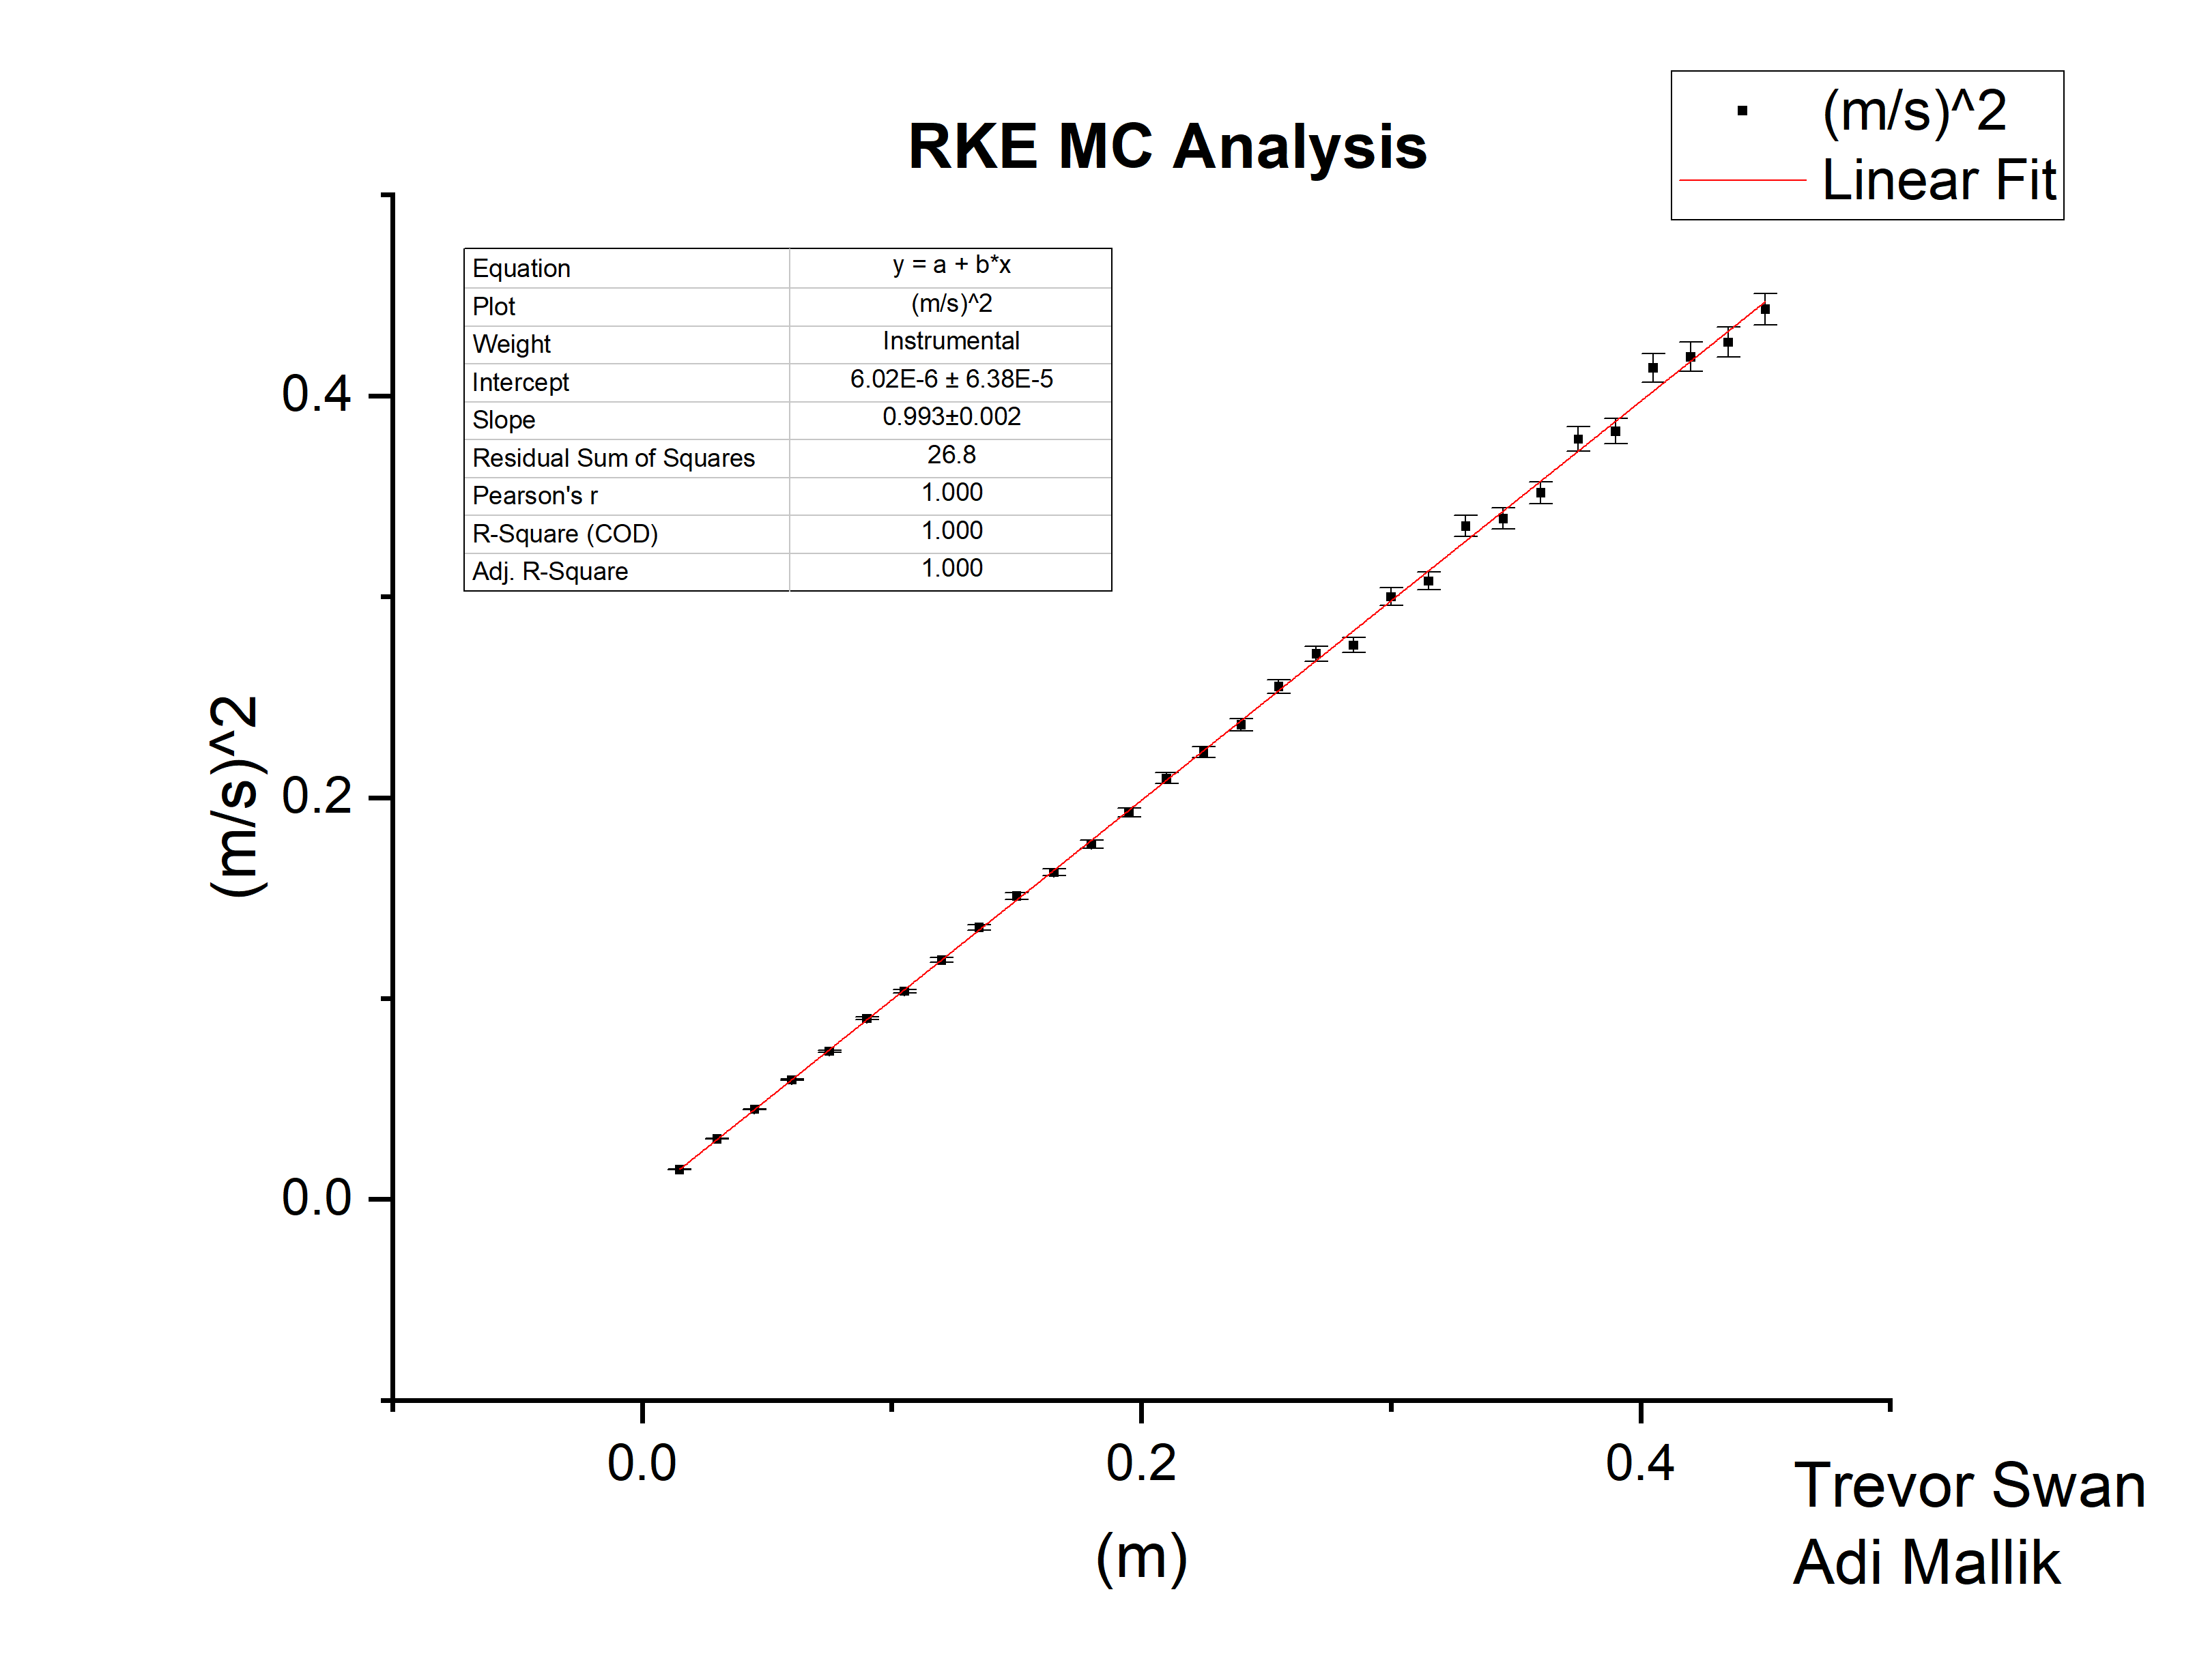
\includegraphics[width=0.8\textwidth]{RKE_MonteC.png}
    \caption{Monte Carlo Simulation}
    \label{MC Plot}
\end{figure}

% Display the massless plot 

\begin{figure} [p]
    \begin{subfigure}
        \centering
        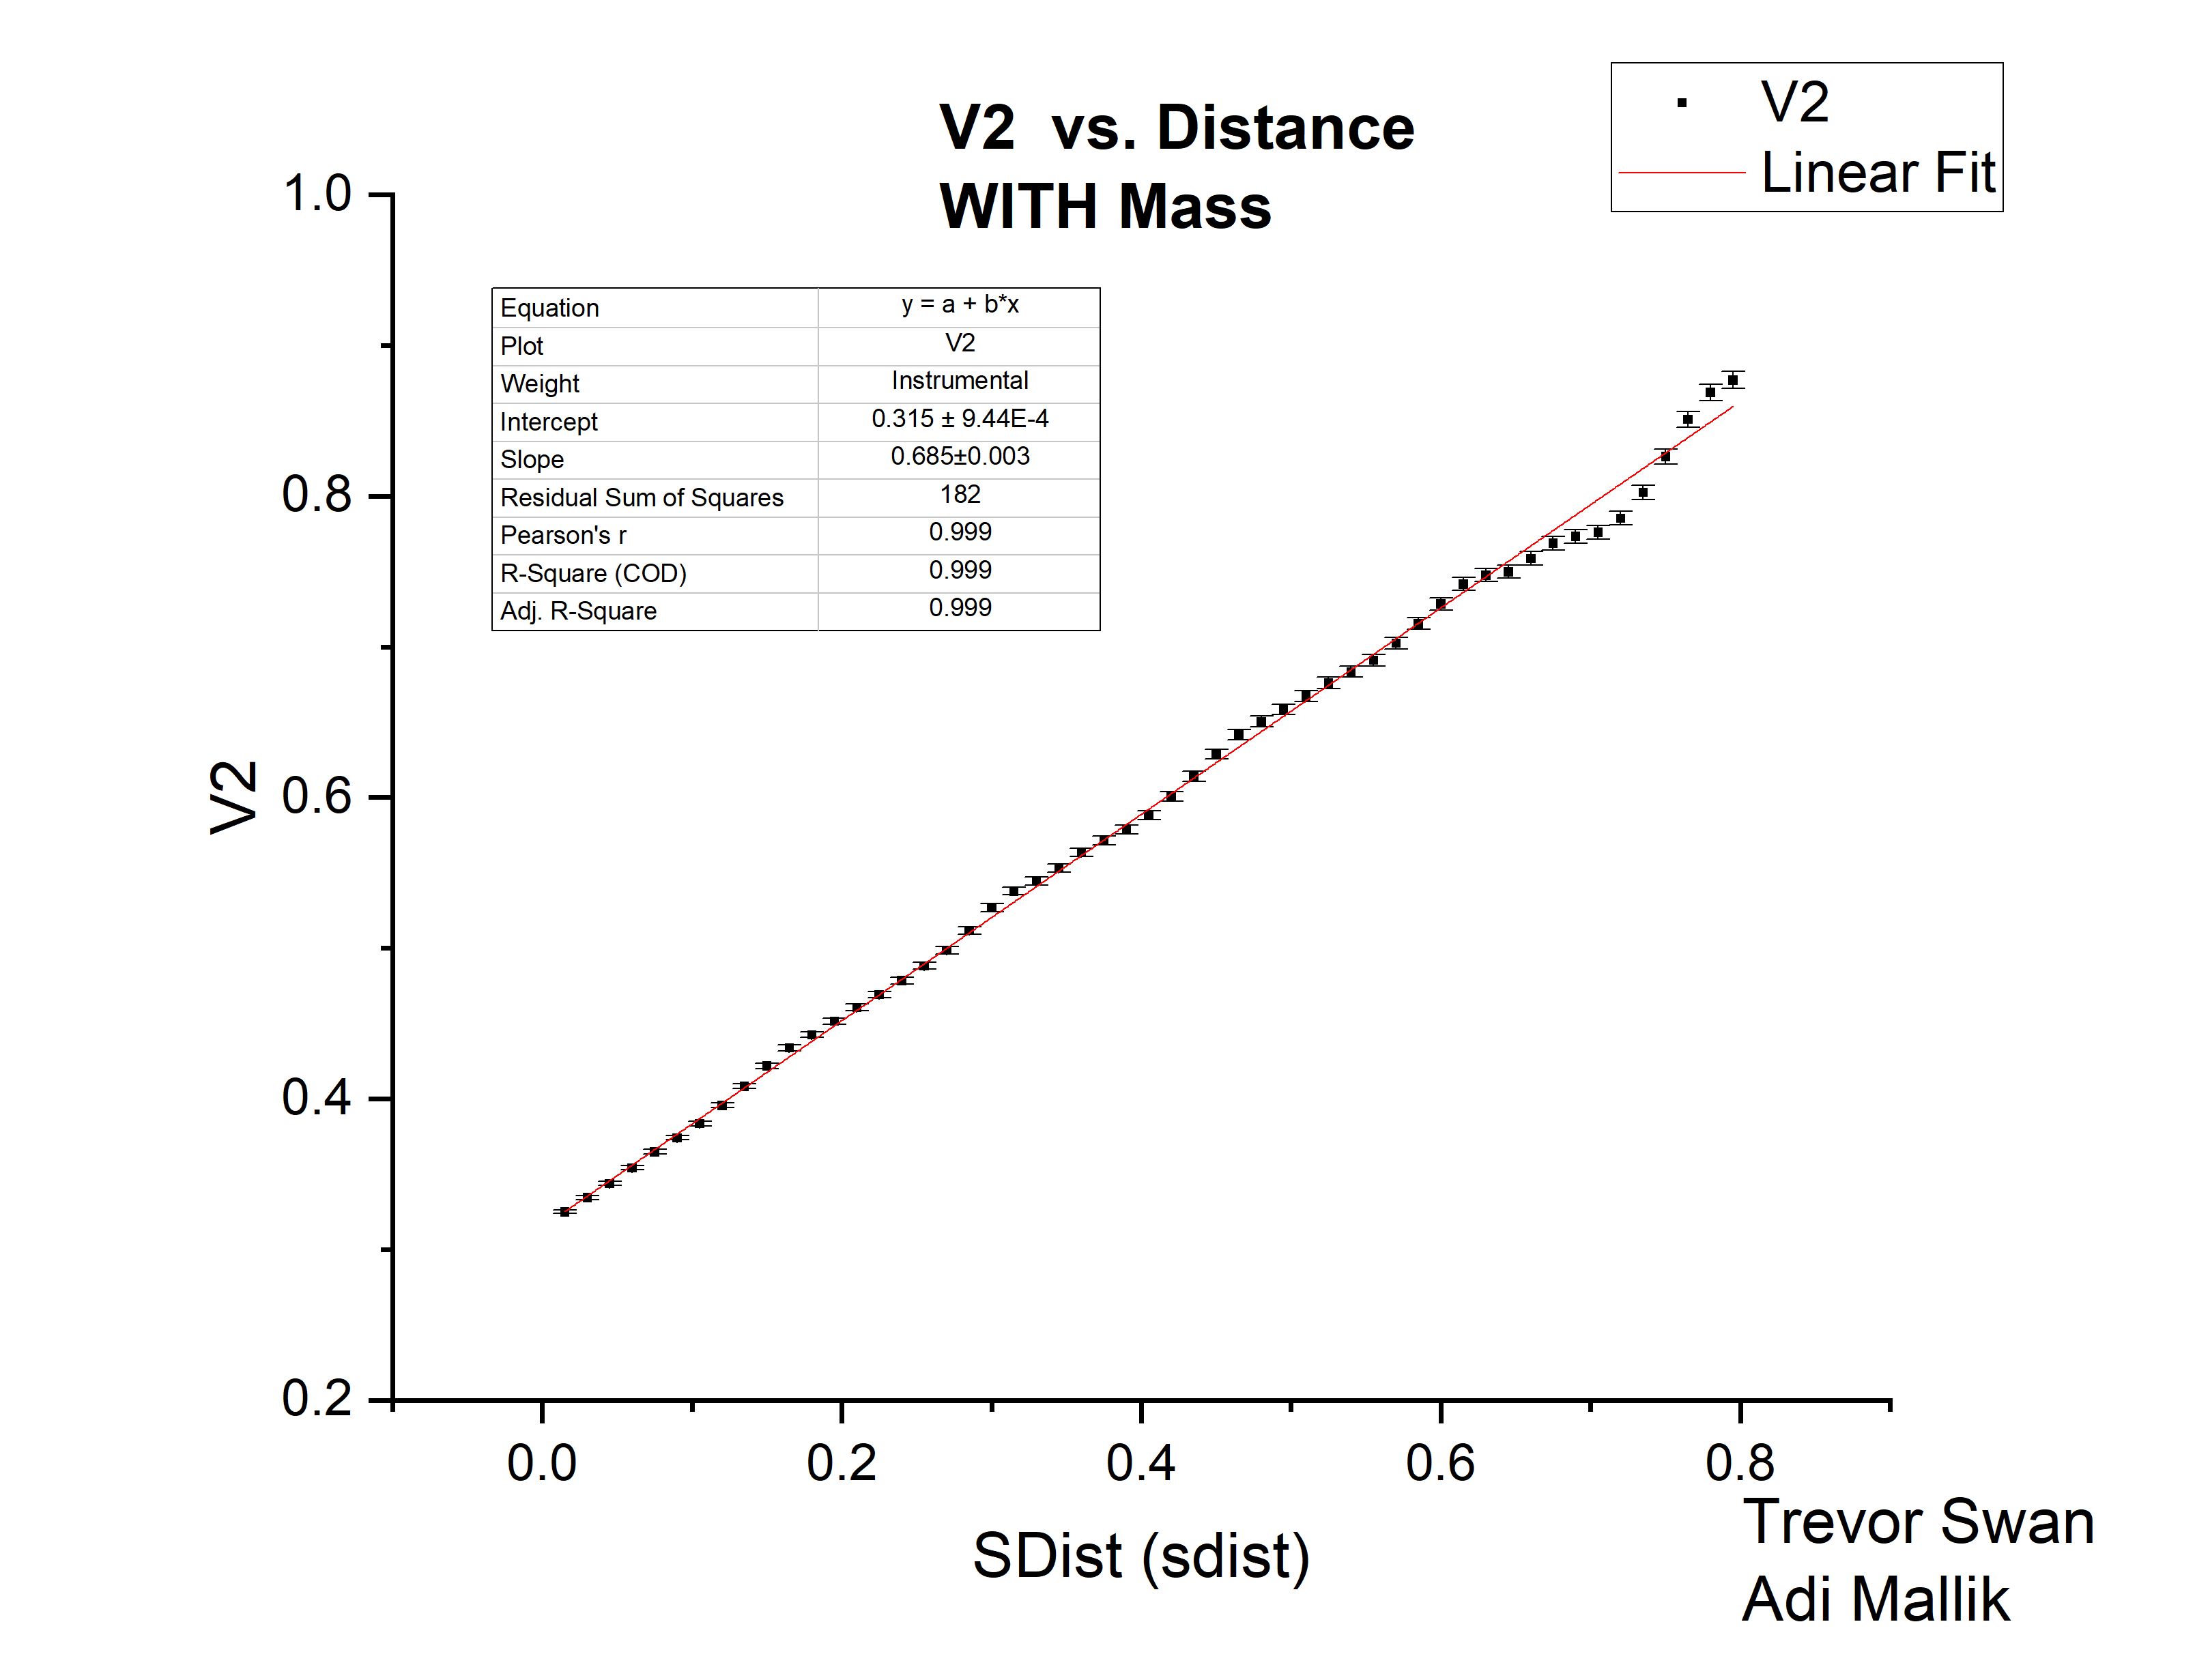
\includegraphics[width=0.8\textwidth]{RKE_withMass.png}
        \caption{$v^2$ vs. $y$ with mass}
        \label{Massed Plot}
    \end{subfigure}
    \begin{subfigure}
        \centering
        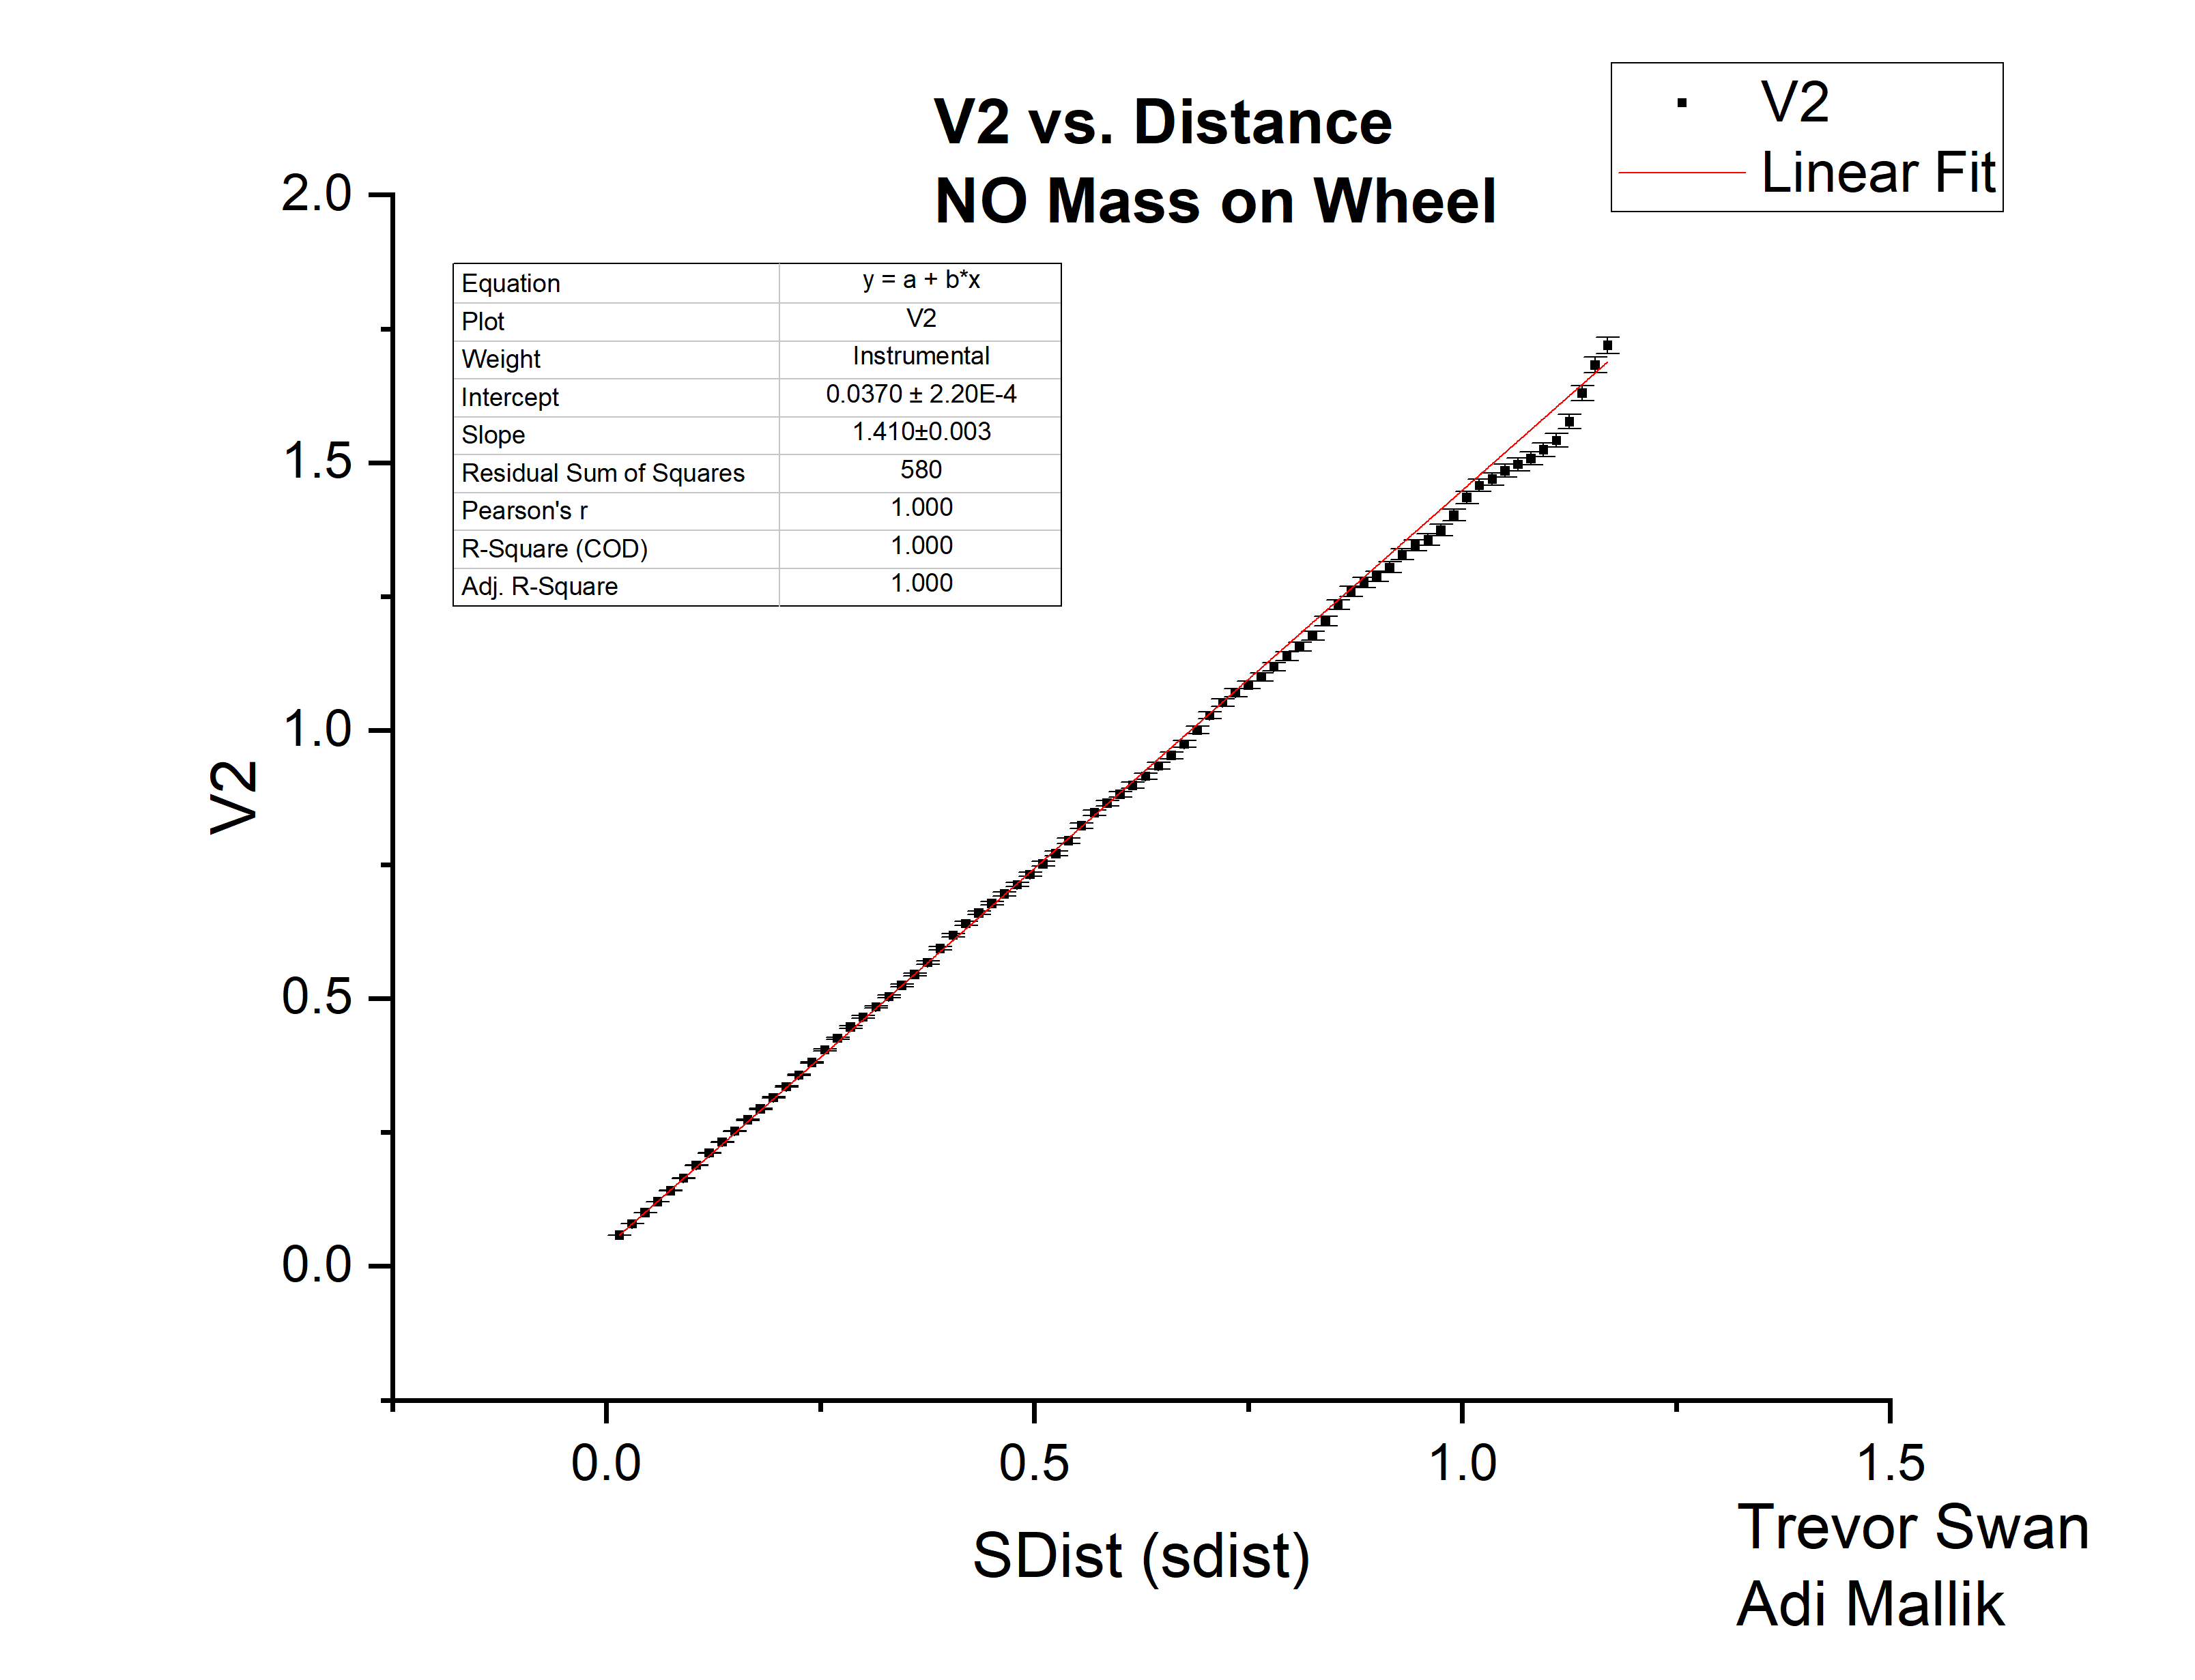
\includegraphics[width=0.8\textwidth]{RKE_noMass.png}
        \caption{$v^2$ vs. $y$ with no mass}
        \label{Massless Plot}
    \end{subfigure}
    
\end{figure}

\end{document}
